\documentclass[letterpaper]{report}
\usepackage[utf8]{inputenc}
\usepackage{amsmath}
\usepackage{amsfonts}
\usepackage{amssymb}
\usepackage{graphicx}
\usepackage[left=1.00in, right=1.00in, top=1.00in, bottom=1.00in]{geometry}

\usepackage{parskip}
\usepackage{enumitem}
\usepackage[table]{xcolor}

\setcounter{secnumdepth}{3}
\renewcommand{\thesection}{\arabic{section}.}
\renewcommand{\thesubsection}{(\alph{subsection})}
\renewcommand{\thesubsubsection}{Solution}

\author{Jacob Huesman}
\title{ECE 343: Signals and Systems, HW \#21, Fall 2017}
\begin{document}
\maketitle


\section{Constant Monthly Contribution}
This problem shares much with the loan problem discussed recently in class. Suppose you would like to retire with 15 million dollars in savings. To make things simple, let’s assume you invest uniform monthly payments for a fixed number of years and that you receive a fixed annual percent yield. Let interest be compounded monthly. Solve this problem using z-transform techniques; I’m not interested in whether you can look up formulas on the internet! 

Using rates rounded to the nearest (non-zero) half percent (e.g., 3 and 4.5 percent are fine, 3.25 percent and 0 percent are not), choose three realistic annual percent yield (interest rates): a low rate $i_{low}$, an average rate $i_{ave}$, and a high rate $i_{high}$. Justify your choices.

Next, consider 3 investment time intervals: $D_{short} = 16$ years, $D_{ave} = 32$ years, and $D_{long} = 48$ years. The number of retirement payments $L$ is clearly going to be 12 times the duration in years $(L = 12D)$. Let $n = 0$ correspond to the first investment contribution, let $n=12D - 1$ be the last investment contribution, and let $n = 12D$ be the time when the retirement account is to have the desired 15 million dollars in savings.

\subsubsection{}
We start by finding three realistic interest rates. For the low rate we choose an interest rate of $i_{low}=0.5\%$. This rate is similar to the $0.38\%$ one can find on the 10 year average annual performance of the Vanguard Federal Money Market Fund. Money Market Funds are very low risk, but also offer a much lower return than most other investments. For the medium rate we choose an interest rate of $i_{med}=6\%$. This rate is similar to the $5.81\%$ one can find on the 17 year average annual performance of the Vanguard 500 Index Fund Admiral Shares which tracks the S\&P 500 Index. Since the S\&P 500 is thought of as a good gauge of the performance of the stock market, it makes a good medium interest rate. This investment is higher risk as the stock market is somewhat volatile. For the high rate we choose an interest rate of $i_{high}=10.5\%$. This rate is similar to the $10.4\%$ one can find on the average annual performance since 1968 of the Vanguard Morgan Growth Fund Investor Shares Mutual Fund, which roughly tracks the Russell 3000 Growth Index. This fund invests in the stock of large and mid sized companies that are predicted to experience above average growth. The risk is a bit higher than that of the S\&P 500 fund as the stocks of fast growing companies are more volatile.

\subsection{Monthly Contribution}
For each interest rate and investment duration, compute the required (fixed) monthly payments $C_{i,D}$ needed to realize the 15 million dollar retirement goal.

\subsubsection{}
We start by creating a difference equation to represent our investment strategy,
\[
	y[n] = \left(1+\frac{i}{12}\right) y[n-1] + C(u[n] - u[n-12D]),
\]
or
\[
	\left(1 - \left(1+\frac{i}{12}\right)E^{-1}\right)y[n] = C(u[n] - u[n-12D]).
\]
Taking the Unilateral Z-Transform of each side we get,
\[
	\left(1 - \left(1+\frac{i}{12}\right)z^{-1}\right)Y(z) = 
	C \left(\frac{z}{z-1} - \frac{z^{-12D+1}}{z-1} \right),
\]
or
\[
	\frac{Y(z)}{z} = C \left(
	\frac{z}{\left(z-1\right)\left(1 - \left(z+\frac{i}{12}\right)\right)} 
	- \frac{z^{-12D+1}}{\left(z-1\right)\left(1 - \left(z+\frac{i}{12}\right)\right)} 
	\right),
\]
where
\[X_{1}(z) = \frac{z}{\left(z-1\right)\left(1 - \left(z+\frac{i}{12}\right)\right)}\]
and 
\[X_{2}(z) = \frac{z^{-12D+1}}{\left(z-1\right)\left(1 - \left(z+\frac{i}{12}\right)\right)}.\]
Notice that $X_{2}(z)$ is just $X_{1}(z)$ with a time shift. We can therefore just solve for $x_{1}[n]$ and then apply the time shift property to get the solution to $x_{2}[n]$. Performing a partial fraction decomposition on $X_{1}(z)$ we get 
\[
	Y_{1}(z) = C\left[\left(-\frac{12}{i} \right)\frac{z}{z-1} 
	+ \left(\frac{12}{i} + 1\right)\frac{z}{z-\left(1+\frac{i}{12}\right)} \right]. 
\]
Taking the Inverse Z-Transform of $Y_{1}(z)$,
\[
	y_{1}[n] = \frac{12C}{i} \left[\left(1+\frac{i}{12}\right)^{n+1} - 1 \right]u[n],
\]
and using the time shift property on $Y_{2}(z)$,
\[
	y_{2}[n] = \frac{12C}{i} \left[\left(1+\frac{i}{12}\right)^{n+1-12D} - 1 \right]u[n-12D],
\]
which gives us
\[
	y[n] = \frac{12C}{i} \left[\left(\left(1+\frac{i}{12}\right)^{n+1} - 1\right) u[n]
    - \left(\left(1+\frac{i}{12}\right)^{n+1-12D} - 1\right) u[n-12D] \right].
\]
In this case, we are trying to solve for $C$, so we let $n = 12D$ and get
\[
y[12D] = \frac{12C}{i} \left[\left(1+\frac{i}{12}\right)^{12D+1} 
- \left(1+\frac{i}{12}\right) \right],
\]
or
\[
y[12D] = \frac{12C}{i} \left(1+\frac{i}{12}\right) \left[\left(1+\frac{i}{12}\right)^{12D} 
- 1 \right].
\]
Solving for $C$,
\[
C_{i,D} = \frac{(i)(y[12D])}{12 \left(1+\frac{i}{12}\right) \left[\left(1+\frac{i}{12}\right)^{12D} 
	- 1 \right]}.
\]
Computing $C_{i,D}$ for the values of $i$ and $D$ specified above, we get the following values:
\begin{table}[h]
	\centering
	\begin{tabular}{|r|r|r|r|}
		\hline 
		i, D & 16 years & 32 years & 48 years \\ 
		\hline 
		0.5\% & \$75,026.66 & \$36,013.91 & \$23,037.34 \\ 
		\hline 
		6.0\% & \$46,483.26 & \$12,892.47 & \$4,472.18 \\ 
		\hline 
		10.5\% & \$30,073.22 & \$4,753.53 & \$866.71 \\ 
		\hline 
	\end{tabular} 
	\caption[Table 1:]{Monthly contribution for particular APYs and investment durations}
\end{table}

\pagebreak
\subsection{Total Amount Invested}
For each interest rate and investment duration, compute the total amount invested (principle).

\subsubsection{}
The monthly contribution is constant for each interest rate and duration, so the amount invested is just the contribution multiplied by the number of months contributed
\[
	P_{i,D} = C_{i,D} * D * 12
\]

Which gives us
\begin{table}[h]
	\centering
	\begin{tabular}{|r|r|r|r|}
		\hline 
		i, D & 16 years & 32 years & 48 years \\ 
		\hline 
		0.5\% & \$14,405,120.13 & \$13,829,342.25 & \$13,269,511.84 \\ 
		\hline 
		6.0\% & \$8,924,786.54 & \$4,950,710.73 & \$2,575,978.17 \\ 
		\hline 
		10.5\% & \$5,774,059.16 & \$1,825,359.28 & \$499,227.07 \\ 
		\hline 
	\end{tabular} 
	\caption[Table 2:]{Total principle invested for particular APYs and investment durations}
\end{table}

\pagebreak
\subsection{Value of Retirement Account}
For each interest rate and investment duration, use MATLAB to plot the value of the retirement account as a function of month over the investment interval (it should end at 15 million dollars). On the same graph using a different line style, plot the principle investment as a function of month over the investment interval (it should always be lower than the other curve). Use subplots so that you can print the nine required graphs on a single piece of paper.

\subsubsection{}
\begin{figure}[h]
	\centering
	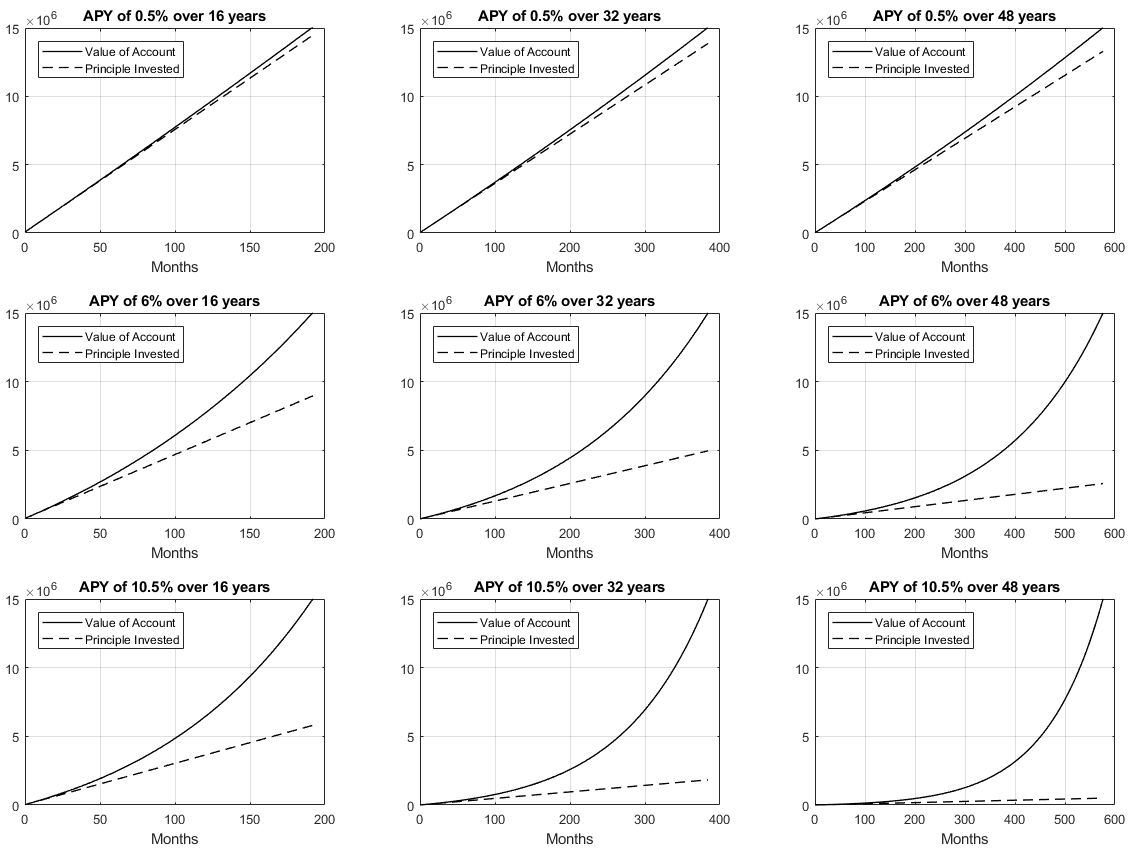
\includegraphics[width=0.95\linewidth]{../hw21_1_cropped}
	\caption{Value of retirement account as a function of month}
\end{figure}

Based on the computations it is clear that the higher the APY and the longer the duration of the investment, the less principle will need to be provided by the investor to reach a desired account value. Although choosing an investment with a decent APY is important, the factor that a young investor has the most control over is the duration of the investment. So the sooner the investor begins investing, the more profitable the investments are likely to be.

\pagebreak
\section{Varying Contribution}
Reconsider Problem 1. Suppose you decide to invest for retirement over 48 years in the following way: you invest $C$ dollars monthly for the first 10 years, $2C$ monthly for the next ten years, $3C$ monthly for the next ten years, and continue this pattern until the last eight years when you are investing $5C$ dollars monthly. This is somewhat realistic in that most people have more disposable income as they progress in their careers. For each of the three interest rates considered in Problem 1, determine the base payment $C_{i}$ to achieve a 15 million dollar retirement. How much is invested in principle? What lessons do you learn here?

\subsubsection{}
This problem can be represented with a difference equation that is very similar to that of Problem 1. The way that interest is calculated and compounded (the impulse response of the system) remains the same, the input just has more components.

Let 
\[
	b[n,v,w] = (u[n-v] - u[n-w])
\]
\[
	y[n] = \left(1+\frac{i}{12}\right) y[n-1] + C\left(b[n,0,120] + 2b[n,120,240] 
	+ 3b[n,240,360] + 4b[n,360,480] + 5b[n,480,576]\right),
\]
or
\[
	y[n] = \frac{12C}{i} h[n] * \left(b[n,0,120] + 2b[n,120,240] 
	+ 3b[n,240,360] + 4b[n,360,480] + 5b[n,480,576]\right)
\]
where 
\[
	h[n] = \left[\left(1+\frac{i}{12}\right)^{n+1} - 1 \right]u[n].
\]
Since the convolution is a linear operator, we can take the convolution of $h[n]$ and each Heaviside unit step function $u[n-m]$, which we already know from Problem 1 to be
\[
	y_{i}[n-m] = \left[\left(1+\frac{i}{12}\right)^{n+1-m} - 1 \right]u[n-m]
\]
where Problem 1 had included the constants $C$, $\frac{12}{i}$ and had set $m=12D$. So
\begin{equation*}
	\begin{split}
		y[n] = \frac{12C}{i}  & [y_{i}[n] - y_{i}[n-120] + 2 (y_{i}[n-120] - y_{i}[n-240]) 
		+ 3 (y_{i}[n-240] - y_{i}[n-360]) \\
		& + 4 (y_{i}[n-360] - y_{i}[n-480] + 5 y_{i}[n-480] - y_{i}[n-576])]
	\end{split}
\end{equation*}
Solving for $C_{i}$
\[
	C_{i} = \frac{(i)y[n]}{12 y_{all}},
\]
where 
\begin{equation*}
	\begin{split}
		y_{all} = & y_{i}[n] - y_{i}[n-120] + 2 (y_{i}[n-120] - y_{i}[n-240]) 
		+ 3 (y_{i}[n-240] - y_{i}[n-360]) \\
		& + 4 (y_{i}[n-360] - y_{i}[n-480] + 5 y_{i}[n-480] - y_{i}[n-576]).
	\end{split}
\end{equation*}

The principle for a particular APY can be calculated as
\[
	P_{i} = 12 * C_{i} * (10 * (1 + 2 + 3 + 4) + 8  * 5)
\]

\pagebreak
Which gives us
\begin{table}[h]
	\centering
	\begin{tabular}{|r|r|r|}
		\hline 
		i &  C & P \\ 
		\hline 
		0.5\% & \$8,160.30 & \$13,709,317.1 \\ 
		\hline 
		6.0\% & \$2,310.26 & \$3,881,251.91 \\ 
		\hline 
		10.5\% & \$573.69 & \$963,814.65 \\ 
		\hline 
	\end{tabular} 
	\caption[Table 1:]{Base monthly contribution and total principle invested for particular APYs}
\end{table}

From the table it is clear to see that with a nominal APY someone on an engineering salary and an upward career trajectory should be able to reach 15 million dollars in their retirement account by retirement. 

\section{ROTH Investments}
Many people contribute to ROTH-variety individual retirement accounts (ROTH IRAs). The maximum allowable ROTH investment is \$5,500 annually. Suppose an recent college graduate is considering two options: a) investing \$5,500 at the beginning of the year from age 22 until age 31 (10 total deposits) and then ignoring the account until retirement, or b) initially making no investment and then investing \$5,500 at the beginning of the year from age 32 until age 64 (33 total deposits). Assuming a historic stock-market average of 7.5 percent APY, which investment option makes most sense? What are the respective account balances when the investor reaches 65 years of age? What is the principle investment in each case? What lessons do you learn here?

For those who want to investigate this problem a little more deeply, why might young investors be better served by a ROTH IRA than a traditional IRA?

\subsubsection{}
The impulse response of this system is similar to that of Problem 1 and 2, the only difference being that the interest is no longer divided by 12 as we are now compounding yearly. Since $\frac{i}{12}$ was just a constant in our impulse response, we can change it to $i$ without doing any additional operations. Our impulse response is then
\[
	h[n] = \left[(1+i)^{n+1} - 1 \right]u[n]
\]
The difference equations can be written as
\begin{equation*}
	\begin{split}
		& y_{1}[n] = (1 + i)(y[n-1] + 5,500(u[n] - u[n-10])),  \\
		& y_{2}[n] = (1 + i)(y[n-1] + 5,500(u[n] - u[n-33])).
	\end{split}
\end{equation*}
Using the impulse response and the convolutions defined in the earlier problems we can rewrite these equations as
\begin{equation*}
	\begin{split}
		& y_{1}[n] = \frac{5,500 (1+i)}{i} [((1+i)^{n+1}-1)u[n] - ((1+i)^{n-9}-1)u[n-10]],  \\
		& y_{2}[n] = \frac{5,500 (1+i)}{i} [((1+i)^{n+1}-1)u[n] - ((1+i)^{n-32}-1)u[n-33]].
	\end{split}
\end{equation*}

\pagebreak
Which gives us:
\begin{table}[h]
	\centering
	\begin{tabular}{|r|r|r|r|}
		\hline 
		Case & Years Investing & Account Balance on Retirement & Principle \\ 
		\hline 
		1 & 43 & \$977,971.00 & \$55,000.00 \\ 
		\hline 
		2 & 33 & \$836,971.33 & \$181,500.00 \\ 
		\hline 
	\end{tabular} 
	\caption[]{Account balances and principles invested in the two scenarios}
\end{table}

Based on the results of this problem, it is clear that the earlier one invests, the more money they stand to earn with less principle investment on their part.

In answer to the last question, a Roth IRA allows investors to pay taxes on deposit instead of on withdrawal. This benefits young investors since the money that accumulates from interest is now tax free. This won't be as appreciable for older investors as there will be less periods for that tax free money to grow. There are obviously other factors to consider, but that is the jist of why it makes sense for young investors.

\end{document}